\section{Исследовательский раздел} 
В данном разделе...

\subsection{Технические характеристики системы}
Исследование проводилось на персональном компьютере со следующими характеристиками:

\begin{itemize}
\item процессор Intel(R) Core(TM) i7-10510U CPU @ 1.80GHz,
\item операционная система Linux (дистрибутив Manjaro Linux, версия ядра Linux 5.13.19-2-MANJARO, архитектура x86-64),
\item 16 Гб оперативной памяти.
\end{itemize}

Вывод разработанных компонентов сохранялся в отдельные текстовые файлы и в дальнейшем, для определения разницы, анализировался с использованием утилиты sdiff.

Для определения того, какие процессы задействуют директорию или файл, использовалась утилита lsof.

\subsection{5 итераций вывода информации о процессах реального времени с разницей в 10 секунд при воспроизведении аудио с использованием MPlayer}
Перед началом исследований было проверено, что аудиофайл не задействован никакими другими процессами, как это показано на рисунке \ref{fig:emptylsof}.

\begin{figure}[H]
	\centering
	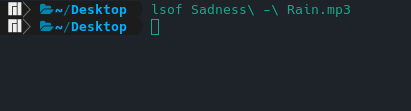
\includegraphics[scale=1]{img/emptylsof.png}
	\caption{Подтверждение того, что файл не задействован никакими другими процессами.}
	\label{fig:emptylsof}
\end{figure}

При запуске проигрывания с использованием MPlayer, утилита lsof указывает на то, что файл используется процессом с именем mplayer (рисунок \ref{fig:mplayerlsof}).

\begin{figure}[H]
	\centering
	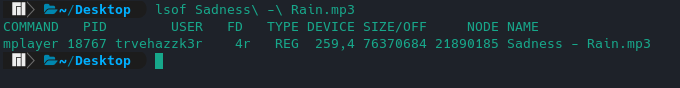
\includegraphics[scale=0.8]{img/mplayerlsof.png}
	\caption{Результат запуска утилиты lsof при воспроизведении файла с использованием Mplayer.}
	\label{fig:mplayerlsof}
\end{figure}

При проведении исследования, первые 10 секунд композиция не запускается. Это связано с тем, что перерывы между получением информации о процессах в модуле заданы данным интервалом времени. Таким образом можно будет наблюдать возможное появление нового процесса, либо динамику изменения полей отдельных task\_struct, отнесенных к задачам реального времени.

В силу того, что файл вывода содержит 1666 строк, его представление здесь нецелесообразно. При анализе результатов было обнаружено, что среди процессов, отнесенных к задачам реального времени, отсутствует процесс с идентификационным номером 18767. Причем, при использовании утилиты pstree у данного процесса обнаруживается лишь один потомок, у которого более нет потомков. Важно отметить также тот факт, что завершение потомка влечет за собой и завершение родительского процесса.

\subsection{5 итераций вывода информации о процессах реального времени с разницей в 10 секунд при воспроизведении аудио с использованием VLC Media Player}
Для достоверности результатов также будет попытка использовать VLC Media Player. Данное исследование проводилось также, как и предыдущее.

\begin{figure}[H]
	\centering
	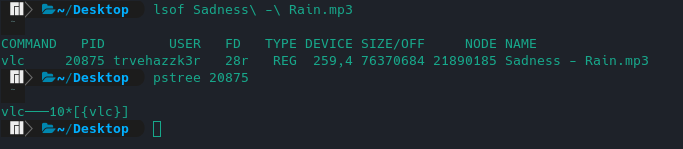
\includegraphics[scale=0.8]{img/vlclsof.png}
	\caption{Результат запуска утилит lsof и pstree при воспроизведении файла с использованием VLC Media Player.}
	\label{fig:vlclsof}
\end{figure}

В силу того, что файл вывода содержит 1666 строк, его представление здесь нецелесообразно. При анализе результатов было обнаружено отсутствие среди проанализированных процессов задачи с идентификационным номером 20875.

\textbf{Таким образом для дальнейшей работы потребуется изменить выборку вывода загружаемого модуля, убрав условие принадлежности задачи к классу процессов реального времени.}

\subsection{5 итераций вывода информации о всех процессах с разницей в 10 секунд при воспроизведении аудио с использованием MPlayer}

\subsection*{Вывод}
В разделе...
